\chapter{Theory}
    \quoteAuthor{It's nice to be right sometimes.}{Peter Higgs}

    Humans have been concerned with the fundamental nature and constituents of matter since as early as eighth century BC, when ancient Indian philosophers, proposed that the objects we experience are collections of particles too small to be seen \cite{indian-atomism}. In sixth century BC, Greek philosophers such as Democritus and Leucippus proposed indivisible building blocks of nature known as ``atoms.'' It wasn't until Dalton in the nineteenth century when scientific modeling of the atomic theory began to take shape \cite{dalton}. Fundamental advances on the nature of atoms and their substructure were made over the next centuries by Mendeleev, Thomson, and Rutherford, among others. Over the course of the latter 1900s, particle theory advanced rapidly and many particles were discovered, forming what was known as the ``particle zoo.'' In order to classify these particles, Gell-Mann and Zweig proposed the quark model in 1964 \cite{quark-model}. In the 1970s Glashow, Weinberg, and Salam put forth the electroweak theory, which gave a model for vector bosons, leading to successful mass predictions of the $W^{\pm}$ and $Z$ bosons confirmed at \gls{CERN} in 1983 \cite{w-discovery, z-discovery}. The collective of these works is known as the \glsfirst{SM} of particle physics, a term first used in 1975 \cite{conceptual-developments-text}. It remains our best model for describing fundamental particles and their interactions\footnote{While the \gls{SM} has been extraordinarily successful in providing experimental predictions, it has several known shortcomings. Notably, the \gls{SM} only explains 3 of the 4 fundamental forces, the exception being gravitation. It does not have an explanation for dark energy or a dark matter candidate. Neutrino flavor oscillation is not predicted by the \gls{SM}, and it predicts neutrino mass to be zero, which has been experimentally disproven \cite{neutrino-oscillation}. The matter-antimatter asymmetry is also not addressed by the \gls{SM}. Nevertheless, it represents our best collective understanding of particle physics.}, successfully predicting the top quark \cite{top-quark}, tau neutrino \cite{tau-neutrino}, and Higgs boson \cite{higgs-discovery-atlas,higgs-discovery-cms}.
    

    \section{The Standard Model}

        The \gls{SM} is a Yang-Mills theory that explains the observed particles in the universe: fermions and bosons. Fermions are the particles which take up space and make up matter. In Section \ref{ssec:fermions}, the two categories of fermions, quarks and leptons, will be discussed. By contrast, interactions between particles are due to exchange of a gauge boson, which are discussed throughout Section \ref{ssec:bosons}.

        Yang-Mills theories are gauge theories, field theories in which the Lagrangian is invariant under local transformations (known as gauge invariance). The group of these transformations is known the symmetry group of the theory. Further, Yang-Mills theories are non-abelian gauge theories, meaning their symmetry group is non-commutative. Noether's theorem \cite{noether} states that every symmetry of nature implies a corresponding conservation law, and the various gauge invariance of the \gls{SM} point toward such conservation laws. In Section \ref{ssec:bosons}, the interactions of the \gls{SM} are shown, each with a gauge invariance and associated force-carrying boson. %TODO: could make this better


        \subsection{Fermions} \label{ssec:fermions}
        Fermions are half-integer spin particles which obey the Pauli Exclusion principle, and thus take up space and make up matter. In the \gls{SM}, there are two types of fermions: quarks and leptons. Each of these can be broken down into three generations of particles, shown in Table \ref{tab:fermions}.

        \noindent{\textbf{Quarks}}\\
        \indent Quarks are fermions which combine to form hadrons. Quarks have several properties:
        \begin{itemize}
            \item Flavor - There are 6 flavors of quarks: up ($u$), down ($d$), strange ($s$), charm ($c$), bottom ($b$), and top ($t$) (from lightest to heaviest). Each quark also has a corresponding anti-quark: anti-up ($\bar{u}$), anti-down ($\bar{d}$), etc. These antiquarks have the same mass, lifetime, and spin as the corresponding quark, but have the opposite sign for their various charge values.
            \item Electric Charge - Quarks either have electric charge of $\frac{2}{3}$ ($u$, $c$, $t$) or $-\frac{1}{3}$ ($d$, $s$, $b$) in units of electron charge, while anti-quarks have the opposite charge. The electric charge of bound states formed by quarks have integer charge, the sum of the constituent quarks.
            \item Color Charge - Each quark has a degree of freedom known as \textit{color charge}\footnote{Quark color is a tool for describing a degree of freedom and has no connection to visible color.}, which can be ``red,'' ``blue,'' or ``green,'' as well as a corresponding anti-color. Color charge is a product of \gls{QCD}, discussed in section \ref{sssec:QCD}, which has a distinct property that particles with color charge cannot be isolated, and must form bound states. This feature is known as \textit{color confinement}. Bound states require a colorless configuration, which may be achieved either through a color-anticolor combination known as mesons, or an (anti)-RGB triplet known as (anti)-baryons. 
        \end{itemize}

        \noindent{\textbf{Leptons}}\\
        \indent The remaining fermions are leptons, which differ from quarks in that they do not have \gls{QCD} color. Each lepton generation contains one charged particle and a neutral counterpart, known as a neutrino. The charged leptons are the electron, muon, and tau (from lightest to heaviest). Table \ref{tab:fermions} also lists the leptons and neutrinos by generation as well as their masses. Each lepton has an associated antilepton as well: the positron, antimuon, and antitau, as well as their antineutrinos. The properties of the antileptons match their corresponding lepton exactly, except the electric charge and lepton number have opposite sign. Lepton number is a conserved quantity in particle interactions and is +1 for all standard leptons, -1 for all antileptons.

        \begin{table}[!thp]
            \centering
            \caption[Fermions in the \gls{SM}, with their masses and charges listed]{Fermions in the \gls{SM}, with their masses and charges listed \cite{pdg}.}
            \begin{tabular}{c|c|c|c|c|}
            \cline{2-5}
                                                           & 1st Generation                                                                & 2nd Generation                                                                                   & 3rd Generation                                                                                 & Charge \\ \hline
            \multicolumn{1}{|c|}{\multirow{2}{*}{Quarks}}  & \begin{tabular}[c]{@{}c@{}}Up ($u$)\\ $m = 2.3^{+0.7}_{-0.5}$ MeV\end{tabular}                       & \begin{tabular}[c]{@{}c@{}}Charm ($c$)\\ $m = 1.275 \pm 0.025$ GeV\end{tabular}                                    & \begin{tabular}[c]{@{}c@{}}Top ($t$)\\ $m = 173.2 \pm 0.7$ GeV\end{tabular}                                    & +2/3   \\ \cline{2-5} 
            \multicolumn{1}{|l|}{}                         & \begin{tabular}[c]{@{}c@{}}Down ($d$)\\ $m = 4.8^{+0.5}_{-0.3}$ MeV\end{tabular}                    & \begin{tabular}[c]{@{}c@{}}Strange ($s$)\\ $m =95\pm 5$ MeV\end{tabular}                                        & \begin{tabular}[c]{@{}c@{}}Bottom ($b$)\\ $m = 4.18 \pm 0.03$ GeV\end{tabular}                                  & -1/3   \\ \hline
            \multicolumn{1}{|l|}{\multirow{2}{*}{Leptons}} & \begin{tabular}[c]{@{}c@{}}Electron ($e^-$)\\ $m = 511$ keV\end{tabular} & \begin{tabular}[c]{@{}c@{}}Muon ($\mu^-$)\\ $m = 105.7$ MeV\end{tabular} & \begin{tabular}[c]{@{}c@{}}Tau ($\tau^-$)\\ $m = 1.8$ GeV\end{tabular} & -1     \\ \cline{2-5} 
            \multicolumn{1}{|c|}{}                         & \begin{tabular}[c]{@{}c@{}}Electron Neutrino ($\nu_e$)\\ $m < 2$ eV\end{tabular}     & \begin{tabular}[c]{@{}c@{}}Muon Neutrino ($\nu_{\mu}$)\\ $m < 0.17$ MeV\end{tabular}                         & \begin{tabular}[c]{@{}c@{}}Tau Neutrino ($\nu_{\tau}$)\\ $m < 15.5$ MeV\end{tabular}                        & 0      \\ \hline
            \end{tabular}
            \label{tab:fermions}
        \end{table}

        Generally, the wave function of a fermion is given by $\psi(x)$, and is a spinor of four components. The motion is described by the relativistic version of the Schr{\"o}dinger equation known as the Dirac equation, given as
        \begin{equation} \label{eqn:dirac}
            (i\gamma'^{\mu}\partial_{\mu}-m)\Psi' = 0
        \end{equation}


        %%%%%% Forces %%%%%%%%        
        \subsection{Bosons and Particle Interactions} \label{ssec:bosons}

        In nature, there are four fundamental forces describing interactions: the strong nuclear force, the weak nuclear force, the electromagnetic force, and the gravitational force. The \gls{SM} models the former three of these forces\footnote{The gravitational force is not modeled by the \gls{SM}. It has relative strength of $10^{-37}$ at $\unit{1}{fm}$. In theories of quantum gravity, it is mediated by the ``graviton'' ($G$), a massless spin-2 particle.}, describing each via a \gls{QFT} corresponding to the exchange of a gauge boson, a particle with integer spin that does not obey the Pauli Exclusion principle. A broad summary of the forces, their bosons, and their associated \glspl{QFT} can be found in Table \ref{tab:forces}, and the following sections will describe the various theories relating to each  interaction.

        \begin{table}[!ht]
            \caption[List of forces described by the \gls{SM}, as well as their associated field theory and gauge boson mediator]{List of forces described by the \gls{SM}, as well as their associated field theory and gauge boson mediator. Relative strength is an order of magnitude estimate at a distance of $\unit{1}{fm}$. The strength of the strong and weak force vary significantly with distance. By coupling constants only (neglecting distance), the weak force is comparable in strength to the \gls{EM} force.}
            \begin{tabular}{l|l|l|l}
            Force & Field Theory & Mediating Boson & Relative Strength      \\ \hline
            Strong Nuclear   & Quantum Chromodynamics  & Gluon ($g$) & $1$ \\
            Electromagnetism & Quantum Electrodynamics & Photon ($\gamma$) & $10^{-3}$ \\
            Weak Nuclear     & Quantum Flavordynamics\tablefootnote{Modern particle physics seldom uses the term quantum flavordynamics. At high energy scales, the weak force and electromagnetic force are interpreted through electroweak theory, which is discussed in Section \ref{sssec:ew-theory}.}  & $W^{\pm}$, $Z$ & $10^{-8}$
            \end{tabular}

            \label{tab:forces}
        \end{table}


        \subsubsection{Quantum Electrodynamics}

        Equation \ref{eqn:dirac}, the Dirac equation, is not gauge invariant. Performing a local gauge transformation on the aforementioned fermion spinor (denoted by $\psi$)
        %
        \begin{equation} \label{eqn:gauge-transform}
            \psi(x) \rightarrow e^{-i\theta(x)}\psi(x),
        \end{equation}        
        %
        for real-valued function $\theta(x)$, will transform the Dirac Lagrangian,
        \begin{equation}
            \mathcal{L} = \bar{\psi}(i \gamma^{\mu}\partial_{\mu}-m) \psi,
        \end{equation}
        which governs the interaction of spin-$\frac{1}{2}$ particles with charge $q$ and mass $m$, like
        \begin{equation}
            \mathcal{L} \rightarrow \mathcal{L} - (\partial_{\mu}\theta)\bar{\psi}\gamma^{\mu}\psi.
        \end{equation}
        %
        In order to impose gauge invariance, we can introduce a vector field. Such a vector field must transform as
        \begin{equation}
            A_{\mu}(x) \rightarrow A_{\mu}(x) + \partial_{\mu}\theta(x),
        \end{equation}
        %
        which has covariant derivative
        \begin{equation}
            D_{\mu} = \partial_{\mu} + iqA_{\mu},
        \end{equation}
        %
        This massless vector field corresponds to the electromagnetic field, and the covariant derivative describes the minimal coupling of the photon, its quanta, to fermions. Applying this vector field to the Dirac Lagrangian gives the \gls{QED} Lagrangian,
        \begin{equation}\label{eqn:qed-lagrangian}
            \mathcal{L}_{QED} = \bar{\psi} (i \gamma^{\mu} D_{\mu} - m)\psi - \frac{1}{4} F_{\mu \nu}F^{\mu \nu}
        \end{equation}
        %
        With $F_{\mu \nu}$, the electromagnetic field tensor, as:
        \begin{equation}\label{eqn:em-field-tensor}
        F_{\mu \nu} = \partial_{\mu}A_{\nu} - \partial_{\nu}A_{\mu}
        \end{equation}
        %
        By this construction, the \gls{QED} Lagrangian is gauge invariant, and symmetric under the transformation described in \ref{eqn:gauge-transform}. This transformation is equivalently thought of as multiplication by a unitary $1 \times 1$ matrix of the $U(1)$ group, meaning \gls{QED} is symmetric under $U(1)$.


        \subsubsection{Quantum Chromodynamics} \label{sssec:QCD}

        \glsfirst{QCD} is the \gls{QFT} corresponding to the strong nuclear interaction, and predicts how quarks and gluons interact. While \gls{QED} corresponds to a $U(1)$ local gauge symmetry, \gls{QCD} corresponds to a $SU(3)$ gauge group, where quarks transform in the fundamental {\bf 3} representation. This representation has eight $3 \times 3$ generators, corresponding to eight gluons, the mediator of the strong force. The dimensionality of the generators mean the wave function has three additional degrees of freedom known as color. Taking the convention of denoting these as ``red'' ($r$), ``green'' ($g$), and ``blue'' ($b$), we can denote the quark spinor as a vector:
        \begin{equation}
            \psi =\begin{pmatrix} \psi_{r} \\ \psi_{b} \\ \psi_{g}\end{pmatrix},
        \end{equation}
        %
        which makes a gauge transformation
        \begin{equation}
        \psi \rightarrow e^{i\theta}e^{-ig {\boldsymbol \lambda\cdot \phi}}\psi.
        \end{equation}
        %
        %todo - clear this up a bit, look at martins notes
        Here $\boldsymbol \lambda$ are the eight Gell-Mann matrices, while ${\boldsymbol \phi} = -{\boldsymbol a}/g$ for vector of length 8 $\boldsymbol a$, and strong coupling constant $g$. This corresponds to the $SU(3)_C$ group ($C$ indicates ``color'').

        In order to achieve invariance under said transformation, the derivative in the Dirac equation is replaced by the covariant derivative 
        \begin{equation}
            D_{\mu} = \partial_{\mu} + ig {\boldsymbol \lambda\cdot {\boldsymbol G_{\mu}}}.
        \end{equation}
        %
        In this, ${\boldsymbol G_{mu}}$ are eight fields, corresponding to eight gluons with various color charge, the mediator of the strong force. This makes the \gls{QCD} Lagrangian
        \begin{equation}
            \mathcal{L}_{QCD} = \bar{\psi}^j (i \gamma^{\mu} D_{\mu}^{jk} - m^{jk})\psi^{k} - \frac{1}{4} F_{\mu \nu}^{a} F^{\mu \nu}_{a},
        \end{equation}
        %
        for mass $m$, indices $j$ and $k$ taking values 1 to 3, and gluon field tensor $F_{\mu \nu}$, given as
        \begin{equation}
            F^{\mu \nu}_{a} = \partial_{\mu} G_{\nu}^a - \partial_{\nu}G_{\mu}^a - g f^{abc} \lambda^a G_{\mu}^b G_{\nu}^c.
        \end{equation}
        %        
        Here $f_{abc}$ are the structure constants associated with the $SU(3)$ group, and indices $a,b,c$ represent the gluons, running from values 1 to 8. Of special note, this tensor contains triplet and quartic gluon self-coupling, a product of the gluon color charge.


        \subsubsection{Electroweak Interaction} \label{sssec:ew-theory}

        In the \gls{SM}, the weak and electromagnetic interactions are interpreted as manifestations of a single force. This unification occurs at energies above $\unit{100}{\GeV}$, and the combined force after unification is known as the electroweak force.

        Electroweak interactions have four mediators, the $W^{\pm}$, $Z$, and $\gamma$, and subsequently four generators. The \gls{SM} would require the masses of these generators to be symmetric: all equal to zero. The $W^{\pm}$ and $Z$, however, have non-zero masses ($m_{W^{\pm}} = \pm80.379\pm0.012$ GeV and  $m_{Z}=91.1876\pm0.0021$ GeV). To reconcile this, a symmetry breaking is introduced, leaving the gauge group electromagnetically invariant. The \gls{SM} of electroweak interactions by Glashow, Weinberg, and Salam \cite{Glashow:1959,Weinberg:1967,Salam1959} contains symmetry breaking:
        \begin{equation}
            SU(2) \times U(1) \rightarrow U(1)_{EM}.
        \end{equation}
        The $SU(2)$ subgroup is weak isospin, where left-handed fermions are doublets, and right-handed fermions are all singlets. The $U(1)$ subgroup is weak hypercharge ($Y$), a conserved quantity. The symmetry breaking described requires the Higgs field, and is known as Electroweak Symmetry Breaking.

%%%%%% Higgs %%%%%%%%                
\section{The Higgs Field and Higgs Boson}

%% New
Consider the $U(1)$ gauge theory with a single gauge field (the photon). The Lagrangian is the second term of Equation \ref{eqn:qed-lagrangian},

\begin{equation}
    \mathcal{L}_{QED} = - \frac{1}{4} F_{\mu \nu}F^{\mu \nu},
\end{equation}
with $F_{\mu \nu}$ defined in Equation \ref{eqn:em-field-tensor}. Adding a massive term to this equation would violate the established local gauge invariance, as the $U(1)$ invariance requires the photon to be massless. If we extend this by adding a complex scalar doublet,
\begin{equation}
\phi = \begin{pmatrix} \phi^+ \\ \phi^0 \end{pmatrix}
    = \frac{1}{\sqrt{2}}\begin{pmatrix}
        \phi_1 + i\phi_2 \\ \phi_3 + i\phi_4,
    \end{pmatrix}
\end{equation}
%
then the Lagrangian and gauge-invariant potential become:
\begin{equation}
    \mathcal{L} = - \frac{1}{4} F_{\mu \nu}F^{\mu \nu} + |D_{\mu}\phi|^2 - V(\phi),
\end{equation}
with:
\begin{equation}
    D_{\mu} = \partial_{\mu} + i \frac{g}{2}\tau \cdot W_{\mu} + i \frac{g'}{2}B_{\mu}Y
\end{equation}
\begin{equation}
    V(\phi) = \mu^2 |\phi|^2 + \lambda (|\phi|^2)^2.
\end{equation}
Where $g$ is the SU(2) gauge coupling, $g'$ is the U(1) gauge coupling, and $Y$ is the U(1) hypercharge. The minima of this potential is known as the vacuum state, and for the minima to be finite, $\lambda$ must be greater than 0. For $\mu^2 >0$, the minima is located at 0, however, for $\mu^2<0$, the potential has minima at:
\begin{equation}
    \phi^\dagger \phi = \frac{v^2}{2},
\end{equation}
where 
\begin{equation}
    v = \sqrt{-\mu^2 / \lambda}.
\end{equation}
This potential is shown (in 2 dimensions) in Figure \ref{fig:higgs-potential}. 

\begin{figure}[!ht]
    \centering
    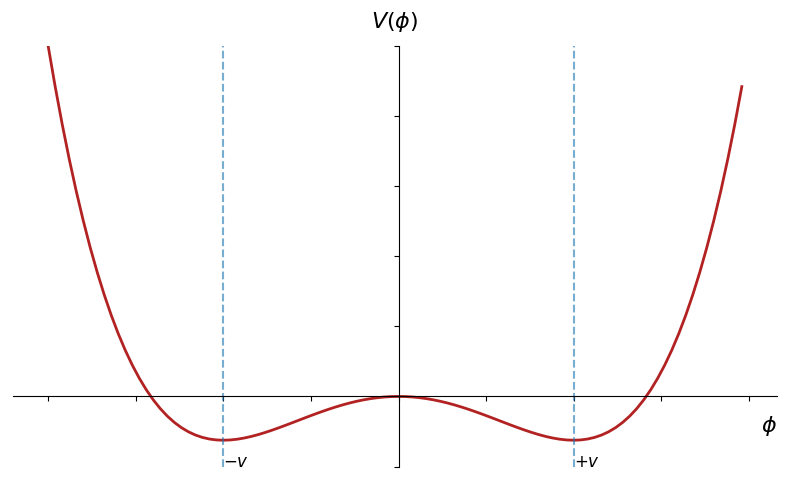
\includegraphics[width=\textwidth]{chapters/chapter1_theory/images/higgs-2d-vev.png}
    \caption[The one-dimensional Higgs potential where $\mu^2 <0$]{The one-dimensional Higgs potential where $\mu^2 <0$. The minima of this curve, known as the Higgs \gls{vev}, is indicated.}
    \label{fig:higgs-potential}
\end{figure}

These minima are degenerate. By convention, we select $v$ to be real, making $\phi_1 = \phi_2 = \phi_3 = 0$, and $\phi_4 = v$.  In making this selection, electroweak symmetry is broken. Unitarity gauge is given by expanding about this minima, making this field:
\begin{equation}
    \phi(x) = \frac{1}{\sqrt{2}} \begin{pmatrix} 0\\ H(x)+v \end{pmatrix}
\end{equation}
%
In this formulation, $H(x)$ represents the Higgs field, and $v$ is known as the \glsfirst{vev}. The contribution to the gauge boson masses from the scalar kinetic energy term of the Lagrangian is then,
\begin{equation}
\frac{1}{2}(0,v)(\frac{1}{2}g\tau \cdot W_{\mu} + \frac{1}{2}g'B_{\mu})^2 \begin{pmatrix}0\\v \end{pmatrix},
\end{equation}
yielding two charged gauge fields and two neutral gauge fields,
\begin{align}
    W^{\pm}_{\mu} &= \frac{1}{\sqrt{2}} ( W_{\mu}^1 \mp i W_{\mu}^2)\\
    Z^{\mu} &= \frac{-g'B_{\mu} + g W_{\mu}^{3}}{\sqrt{g^2 + g'^{2}}}\\
    A^{\mu} &= \frac{gB_{\mu} + g' W_{\mu}^{3}}{\sqrt{g^2 + g'^{2}}}.
\end{align}
This provides a prediction the prediction of the gauge boson masses:
%
\begin{equation}
    m^2_W = \frac{g^2 v^2}{4}, \hspace{1cm} m^2_Z = \frac{(g^2 +g'^2)v^2}{4}, \hspace{1cm} m_{A} =0,
\end{equation}
%
which agrees with experimental values when the \gls{vev} is $\unit{246}{\GeV}$. Since the massless gauge boson must couple with strength $e$, this gives the weak mixing angle $\theta_{W}$,
\begin{align}
    e &= g \sin{\theta_W} \\
    e &= g' \cos{\theta_W}
\end{align}
In unitarity gauge, the Higgs potential takes the form:
\begin{equation}
    V(h) = \lambda v^2 h^2 + \lambda v h^3 + \frac{\lambda}{4}h^4,
\end{equation}
%
indicating self-interactions with the Higgs boson. The second term gives rise to the trilinear coupling, while the third indicates the Higgs quartic coupling. These couplings imply the existence of $hhh$ and $hhhh$ verticies, respectively. The Higgs boson mass can also be derived as $m_h = \sqrt{2\lambda}v$. 


%%%%%% Di-Higgs %%%%%%%%                
\section{Di-Higgs Production} \label{sec:diHiggs}

Observing the trilinear coupling directly probes electroweak symmetry breaking, and provides a precision test electroweak theory. For a direct probe\footnote{Through loop corrections, mono-Higgs searches can provide an indirect handle on the trilinear coupling. ATLAS has published one such analysis with $\unit{80}{\invfb}$, found in Reference \cite{monohiggs-selfcoupling}. When making the assumption that all other Higgs couplings are as predicted by the \gls{SM}, this analysis finds the observed (expected) $95\%$ C.L. interval on the trilinear coupling to be $-3.2 < \kappa_\lambda <11.9$   $(-6.2 < \kappa_\lambda <14.4)$. }, production modes resulting in pair and triplet Higgs production must be studied. The cross-section of such production modes, however, is quite small. Triplet production of Higgs bosons occurs at a rate 6 orders of magnitude less frequently than mono-Higgs production, and is not feasible to study at the \gls{LHC}. Pair production is 3 orders of magnitude more rare than mono-Higgs production, but over the full \gls{LHC} lifetime, a handle on the trilinear self-coupling may be achievable.

The analysis presented in this thesis is one such search for di-Higgs production, specifically where one of the produced Higgs bosons decays to a pair of photons, and the other to a $b\bar{b}$ pair.

\subsection{Higgs Boson Pair Production in the Standard Model}
In the standard model, several production modes pair produce Higgs bosons. \gls{ggF} is the most dominant with a cross-section accounting for over $90\%$ of di-Higgs production, described in section \ref{sssec:ggfHH}. The next most dominant is Vector Boson Fusion, which is responsible for just over $5\%$ of di-Higgs production and is described in section \ref{sssec:vbfHH}. The remaining production modes, $VHH$, $ttHH$, and $tjHH$ collectively comprise less than 5\% of di-Higgs production, and have a cross-section too small to make a meaningful contribution to the presented analysis.

\subsubsection{Gluon-Gluon Fusion} \label{sssec:ggfHH}

The predominant di-Higgs production mode is \gls{ggF}, in which the production is mediated by a quark loop. In the \gls{SM}, this proceeds through two diagrams at tree level, where the quark loop either forms a box or a triangle. The former directly pair produces two Higgs bosons while the latter pair produces via a virtual Higgs boson, making it sensitive to the Higgs self-coupling, $\lambda_{HHH}$. These two diagrams interfere destructively. QCD corrections to this process are known to \gls{NLO}, and can double the cross-section from the \gls{LO} value. Furthermore, \gls{NNLO} corrections are known in the large top mass limit\footnote{The large top mass limit approximates $m_t$ to be large compared to the partonic center-of-mass collision energy and $m_H$, in order to approximate \gls{QCD} corrections to HH production. This approximation provides a poor description of of the total cross section and kinematics \cite{large-mt}.} and represent a $\sim 20\%$ increase from the \gls{NLO} prediction. At $\unit{13}{\TeV}$, the cross-section for \gls{ggF} production is $31.05^{+2.2\%}_{-5.0\%} \pm 3.0\%$\footnote{The first (upper and lower) uncertainties refer to scale uncertainties, the second is PDF + $\alpha_s$ uncertainty.}  \cite{hh-crosssections}.

\begin{figure}[!thp]
    \centering
    \begin{minipage}[c]{.40\textwidth}
        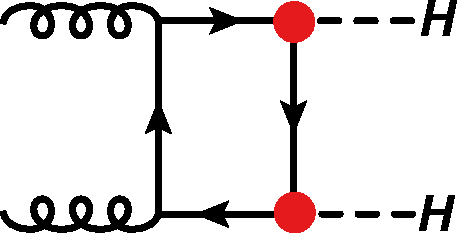
\includegraphics[width=\textwidth]{chapters/chapter1_theory/images/hh_box.pdf}
    \end{minipage}
    \hspace{0.09\textwidth}
    \begin{minipage}[c]{.40\textwidth}
        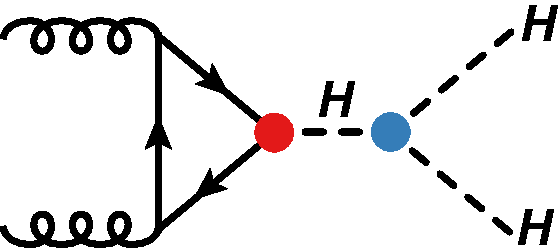
\includegraphics[width=\textwidth]{chapters/chapter1_theory/images/hh_triangle.pdf}
    \end{minipage}

    \caption[Tree level Feynman diagrams for nonresonant \gls{ggF} $HH$ production]{Tree level Feynman diagrams for nonresonant \gls{ggF} $HH$ production. The left is the ``box'' diagram, which is not sensitive to the Higgs trilinear coupling. The right is the ``triangle'' diagram, which is sensitive to the Higgs trilinear coupling, $\lambda_{HHH}$, via the interaction between the virtual Higgs boson and the pair produced di-Higgs system labeled by the blue vertex.}
    \label{fig:ggf_feyn}
\end{figure}

\subsubsection{Vector Boson Fusion} \label{sssec:vbfHH}
The second-most dominant $HH$ production mode is \gls{VBF} ($qq \rightarrow HHqq$), in which two quarks scatter via the exchange of a virtual vector boson, $W^\pm$ or $Z$ (generally denoted $V$), and from that boson, a di-Higgs system is produced. This proceeds via three Feynman diagrams at tree level, shown in Figure \ref{fig:vbf_feyn}. At $\unit{13}{\TeV}$, the cross-section for \gls{VBF} production is $1.73^{+0.03\%}_{-0.04\%} \pm 2.1\%$\cite{hh-crosssections}.

\begin{figure}[!thp]
    \begin{minipage}[c]{.31\textwidth}
        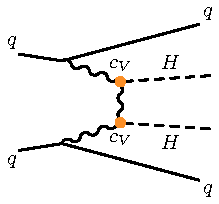
\includegraphics[width=\textwidth]{chapters/chapter1_theory/images/vbf_cv.pdf}
    \end{minipage}
    \begin{minipage}[c]{.31\textwidth}
        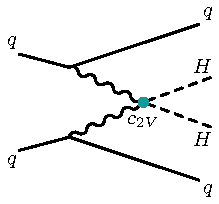
\includegraphics[width=\textwidth]{chapters/chapter1_theory/images/vbf_c2v.pdf}
    \end{minipage}
    \begin{minipage}[c]{.31\textwidth}
        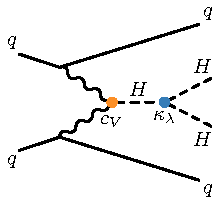
\includegraphics[width=\textwidth]{chapters/chapter1_theory/images/vbf_klambda.pdf}
    \end{minipage}

    \caption[Tree level Feynman diagrams for nonresonant \gls{VBF} $HH$ production]{Tree level Feynman diagrams for nonresonant \gls{VBF} $HH$ production \cite{vbf_4b}.}
    \label{fig:vbf_feyn}
\end{figure}

The coupling denoted $c_V$ is the interaction between two vector bosons and a Higgs boson. This coupling has constraints from mono-Higgs analyses, measured at $1.21^{+0.22}_{-0.21}$ the \gls{SM} value \cite{higgs-measurements}. The coupling denoted $\kappa_{\lambda}$ is again the Higgs trilinear coupling, meaning that the \gls{VBF} production mode offers sensitivity to this vertex as well. Phenomenology studies at parton level have shown the sensitivity in the \gls{VBF} mode to provide a competitive handle on $\kappa_{\lambda}$ \cite{vbf_lambda}. The coupling denoted $c_{2V}$ is the interaction between two vector bosons and two Higgs bosons. \gls{VBF} $HH$ searches offer a unique handle on this vertex, previously entirely unconstrained.

Despite the low cross-section of \gls{VBF} production, the unique kinematics make the channel appealing for searches. The diphoton \gls{VBF} channel contributed to the 2012 single Higgs boson discovery \cite{higgs-discovery-atlas}. Notably, the \gls{VBF} quarks yield a high $m_{jj}$ system and are largely separated in $\eta$. The kinematics of \gls{VBF} di-Higgs production are similar to that of mono-Higgs. The major difference is that mono-Higgs searches take advantage of the low central jet activity by applying a veto. In $HH \rightarrow \gamma \gamma b\bar{b}$, however, the $H \rightarrow b\bar{b}$ system causes central jet activity, making such a veto impossible.


\subsection{Production Beyond the Standard Model}

Due to the small cross-section of $HH$ production, the current ATLAS dataset does not have sensitivity to \gls{SM} production. An enhancement to the cross-section, however, may be noticeable in the dataset and would indicate the presence of physics \gls{BSM}. There are a variety of scenarios in which this could occur, both through a resonance and through non-resonant enhancements.

\subsubsection{Non-Resonant BSM Production}

Non-resonant enhancements to the $HH$ cross-section could occur through two major routes: deviations in couplings from \gls{SM} value, or the presence of couplings not predicted by the \gls{SM}.

\noindent{${\boldsymbol \kappa_{\lambda}}$}\\
\indent Deviations from the \gls{SM} prediction of the Higgs trilinear coupling can cause enhancements to the cross section, which may be observable at the current \gls{LHC} dataset. The cross section is minimized at 2.45 times the \gls{SM} value, in which the destructive interference between the box and triangle diagrams is maximized. The cross section for each production mode as a function of the coupling strength can be seen in Figure \ref{fig:klambda-xsec}.

\begin{figure}[!ht]
    \centering
    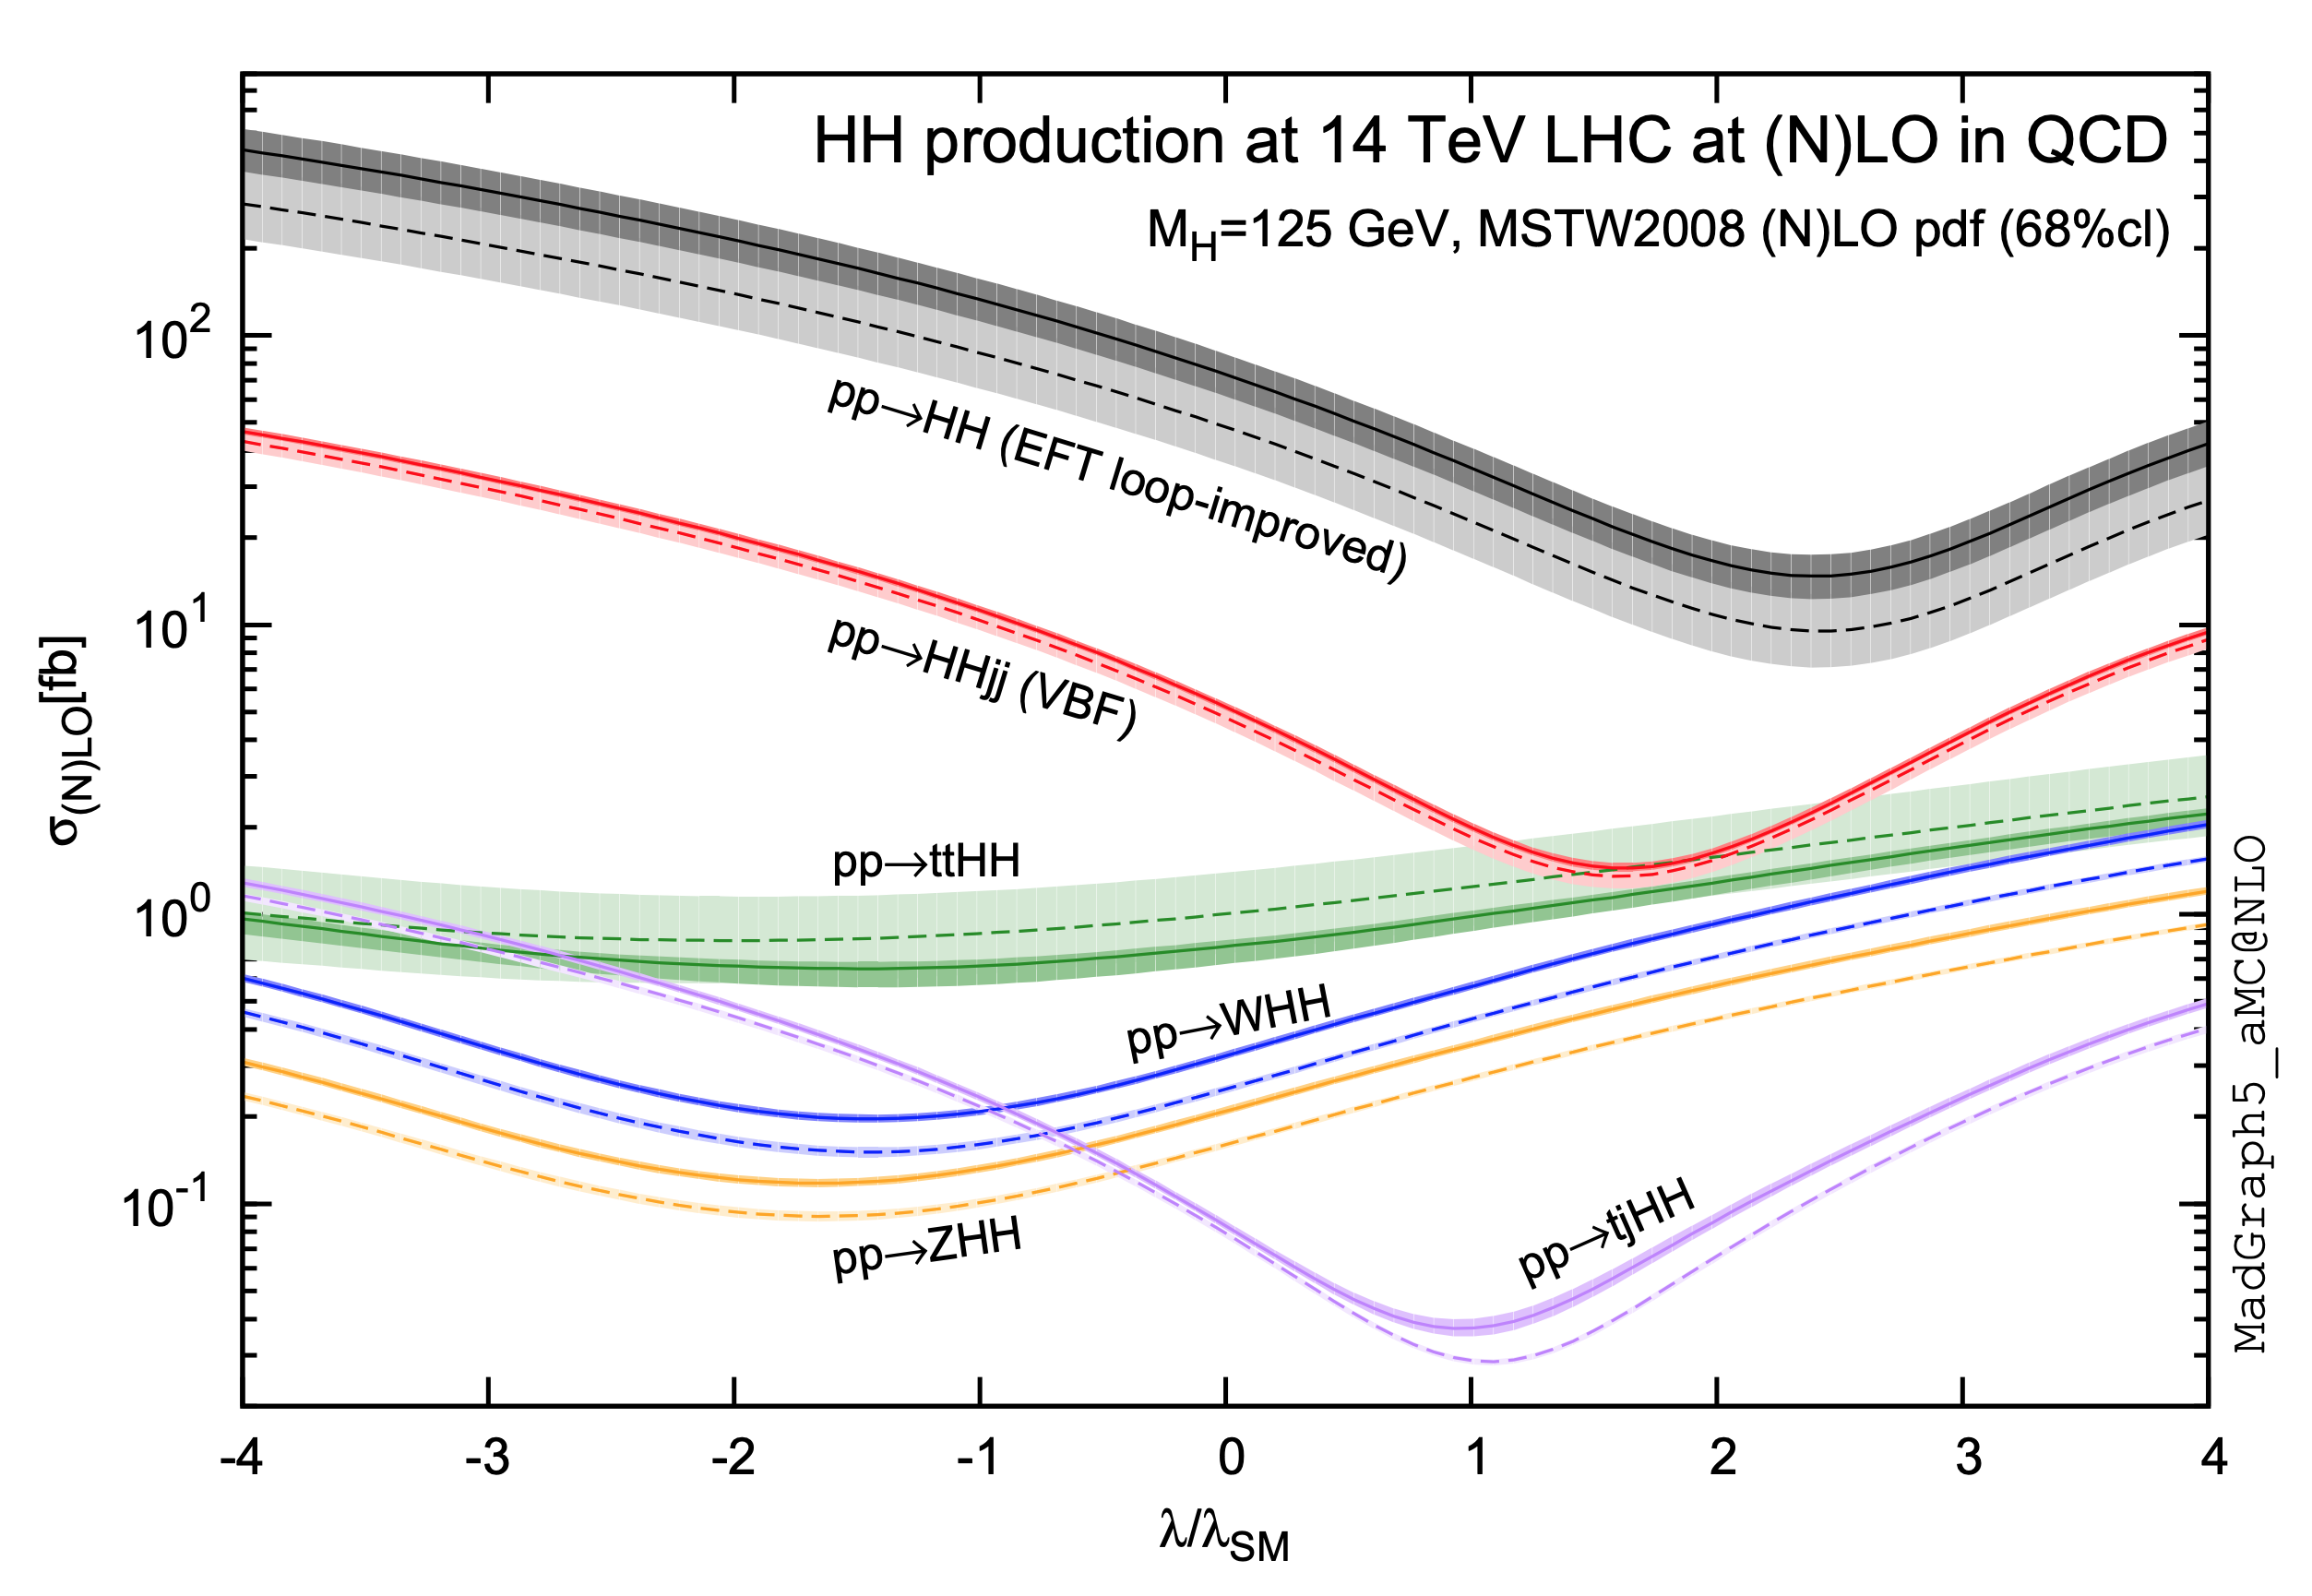
\includegraphics[width=.7\textwidth]{chapters/chapter1_theory/images/klambda-xsec.png}
    \caption[LO and NLO cross-sections for the various $HH$ production modes as a function of the Higgs trilinear coupling]{\gls{LO} (dashed lines, light-color bands) and \gls{NLO} (solid lines, dark-color bands) cross-sections for the various $HH$ production modes as a function of the Higgs trilinear coupling, normalized to the standard model coupling value. Uncertainties represent scale and PDF uncertainties, added linearly \cite{klambda-xsec}.}
    \label{fig:klambda-xsec}
\end{figure}

\noindent{${\boldsymbol c_{2V}}$}\\
\indent The \gls{VBF} $HH$ production mode offers sensitivity to the $hhVV$ vertex, and any deviations from \gls{SM} expectations for this coupling would lead to a significant enhancement in the $HH$ cross-section. At a factor of 2 times the standard model coupling strength, the cross-section increases by two orders of magnitude (shown in Figure \ref{fig:c2v-xsec}), allowing for an enhancement visible in the current \gls{LHC} dataset \cite{vbfhh}.


\begin{figure}[!ht]
    \centering
    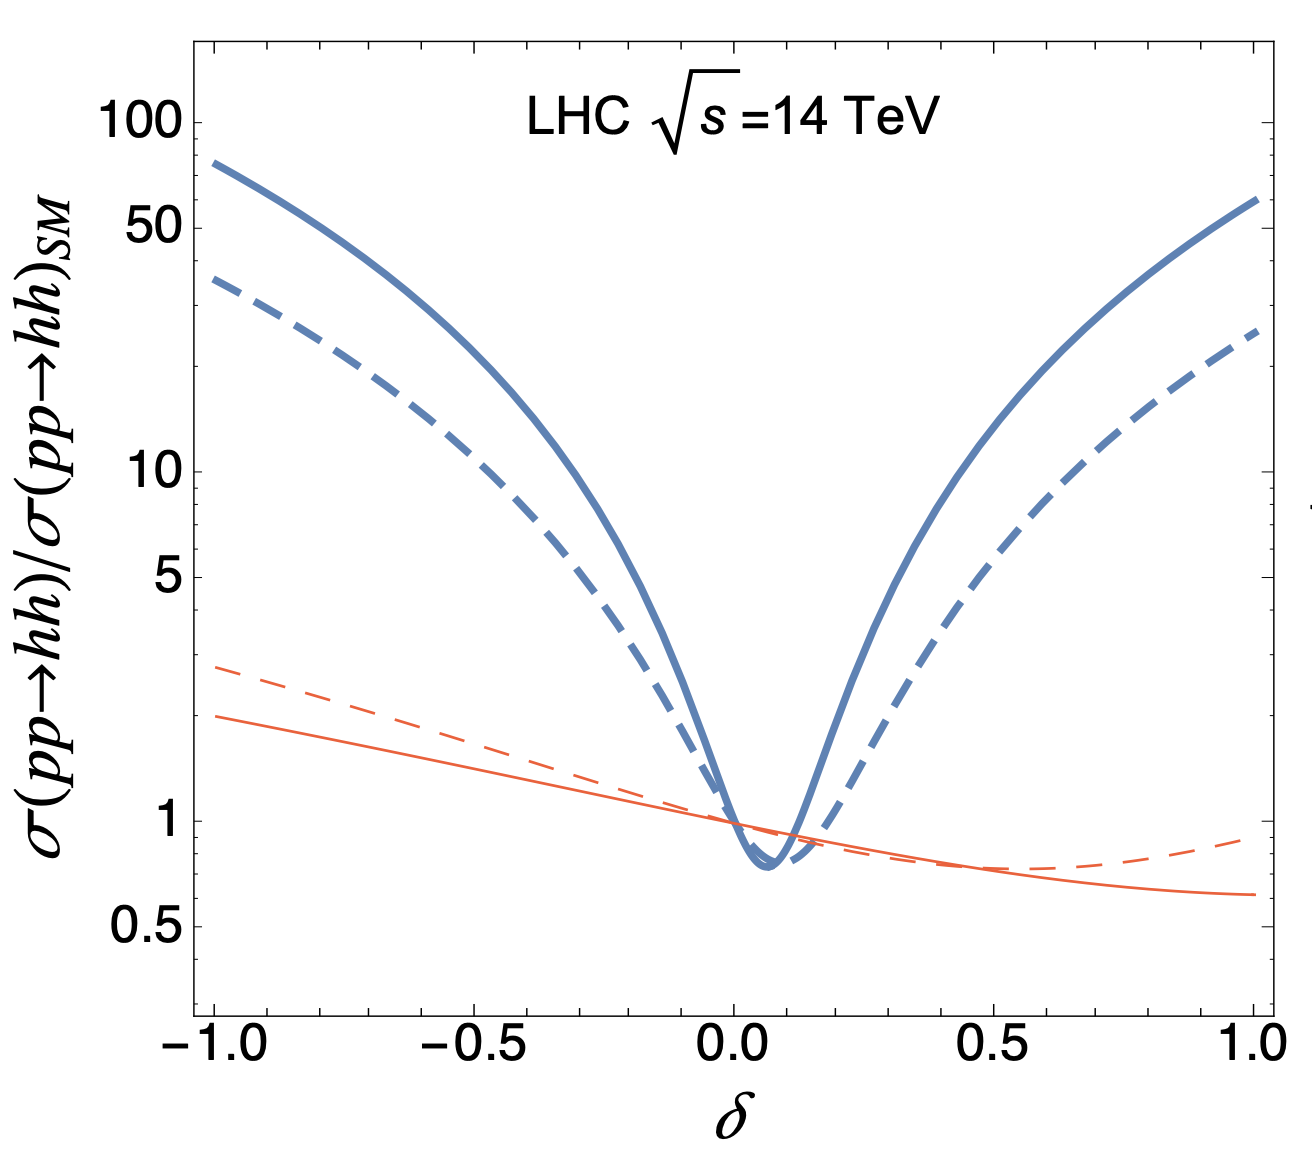
\includegraphics[width=.7\textwidth]{chapters/chapter1_theory/images/coupling_xsec.png}
    \caption[The VBF HH cross-section as a function of coupling deviation from the \gls{SM} prediction]{The VBF HH cross-section as a function of coupling deviation from prediction, in units of the \gls{SM} value ($\delta=c-c_{SM}$ for coupling, $c$. I.e. $\delta=0$ corresponds to the \gls{SM} prediction, $\delta=1$ is twice the \gls{SM} prediction). The solid blue line shows deviations in the $c_{2V}$ vertex, $\delta_{c_{2V}}$, while the red line shows deviations for the $c_{3}$ vertex, $\delta_{\kappa_{\lambda}}$. The dashed lines represent the cross-section after simple analysis cuts presented in Reference \cite{vbfhh}.}
    \label{fig:c2v-xsec}
\end{figure}



\subsubsection{Resonant BSM Production}

Several \gls{BSM} theories predict new particles that would decay to a pair of Higgs bosons, which would result in a resonant enhancement to the $HH$ cross-section. Notably, \glspl{THDM} extend the Higgs sector with the presence of a heavy scalar doublet \cite{THDM}. Among these models are the minimal supersymmetric extension of the \gls{SM} \cite{mssm}, twin Higgs models, and composite Higgs models \cite{compositeHiggs}. The analysis presented in this thesis is model-independent, searching for enhancements to the $HH$ cross section through the presence of a generic scalar particle.

\noindent\textbf{\gls{ggF}}\\
\indent In \gls{ggF} production, the resonance would be present through the generic scalar coupling to the triangle diagram, which subsequently decays into the $HH$ pair. As a result, this resonance would be observed as an enhancement to the $HH$ cross section, as this production is not modeled in the \gls{SM}. A sample Feynman diagram for such a resonance can be seen in Figure \ref{fig:ggf-resonant}.


\begin{figure}[!ht]
    \centering
    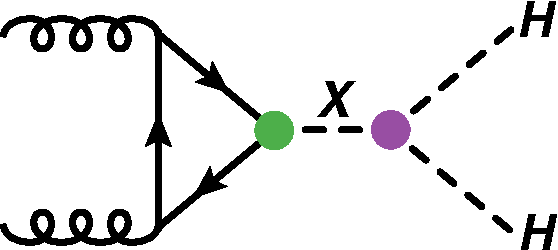
\includegraphics[width=.45\textwidth]{chapters/chapter1_theory/images/hh_res_ggf.pdf}
    \caption{A Feynman diagram for resonant ggF  $HH$ production. In the analysis presented, $X$ takes the form of a generic scalar to remain model-independent.}
    \label{fig:ggf-resonant}
\end{figure}

\noindent\textbf{VBF}\\
\indent Similarly to the searches for resonant ggF Higgs boson pair production, \gls{VBF} $HH$
production involving an intermediate resonance may be considered. This kind of search would be complementary to the ggF searches, as in this case the vector bosons are the ones coupling to the new resonance, which then decays to a pair of Higgs bosons, as depicted in Figure \ref{fig:vbf-resonant}. However, this production mode is not
particularly well studied (Reference \cite{res_vbf} presents an analysis in the context of a model with warped extra dimensions), since its very small cross section poses a question on the ability of the LHC to impose significant constraints through this type of search.

\begin{figure}[!ht]
    \centering
    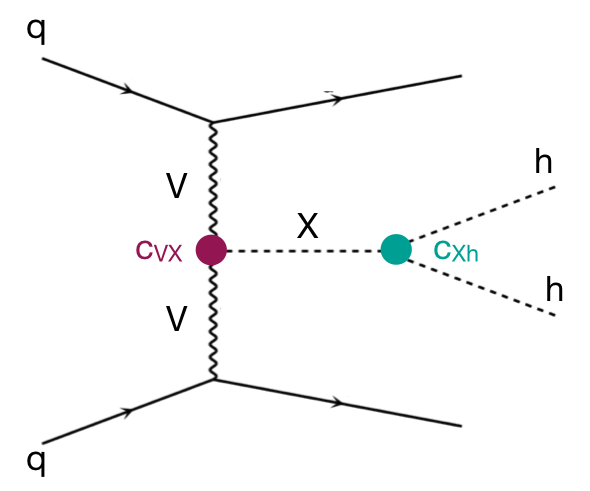
\includegraphics[width=.45\textwidth]{chapters/chapter1_theory/images/vbf_resonant.png}
    \caption{A Feynman diagram for resonant VBF $HH$ production.}
    \label{fig:vbf-resonant}
\end{figure}

\subsection{Decay in the Standard Model}

Due to the short lifetime of the Higgs boson, measurements and searches are performed by studying its decay particles. The Higgs directly couples to all massive particles, and decays directly to any such massive particles provided conservation laws are followed. Additionally, it can decay to massless particles via virtual loops, but as a result, these branching ratios are relatively small. The \gls{SM} Higgs branching ratios are shown in table \ref{tab:higgs-decays}. 

\begin{table}[!thp]
    \centering
    \caption[Branching ratios for the \gls{SM} Higgs boson]{Branching ratios for the \gls{SM} Higgs boson \cite{pdg}.}
    \begin{tabular}{c|c}
        Channel & Branching Ratio \\
        \cline{1-2}
        $H \rightarrow b\bar{b}$ & $57.5 \pm 1.9$\\
        $H \rightarrow WW^*$ & $21.6 \pm 0.9$\\
        $H \rightarrow gg$ & $8.56 \pm 0.86$\\
        $H \rightarrow \tau^+ \tau^-$ & $6.30 \pm 0.36$\\
        $H \rightarrow c\bar{c}$ & $2.90 \pm 0.35$\\
        $H \rightarrow ZZ^*$ & $2.67 \pm 0.11$\\
        $H \rightarrow \gamma\gamma$ & $0.228 \pm 0.011$\\
        $H \rightarrow Z\gamma$ & $0.155 \pm 0.014$\\
        $H \rightarrow \mu^+ \mu^-$ & $0.022 \pm 0.001$
    \end{tabular}
    \label{tab:higgs-decays}
\end{table}

In di-Higgs searches, properties of both Higgs decays must be considered. Branching ratios for various combinations of $HH$ decays are shown in Figure \ref{fig:hh-brs}. The already small $HH$ cross section motivates searches to target high branching ratio decay modes, thus the three primary channels of study all incorporate the $H\rightarrow b\bar{b}$ decay. The $b\bar{b}b\bar{b}$ decay channel has highest possible branching ratio at $33.9\%$, but has significant challenges presented by triggering and a large QCD background. The $b\bar{b}\tau \tau$ has the third largest branching ratio at $7.3\%$, and benefits from a much smaller \gls{SM} background than the $b\bar{b}b\bar{b}$ channel, primarily $t\bar{t}$ and $Z\rightarrow \tau^+ \tau^-$ + jets. Last the $b\bar{b} \gamma \gamma$ channel, presented in this thesis, has just a $0.3\%$ branching ratio, but takes advantage of the excellent $H\rightarrow \gamma\gamma$ mass resolution, as well as the clean diphoton trigger and photon reconstruction efficiency.

\begin{figure}[!htp]
    \centering
    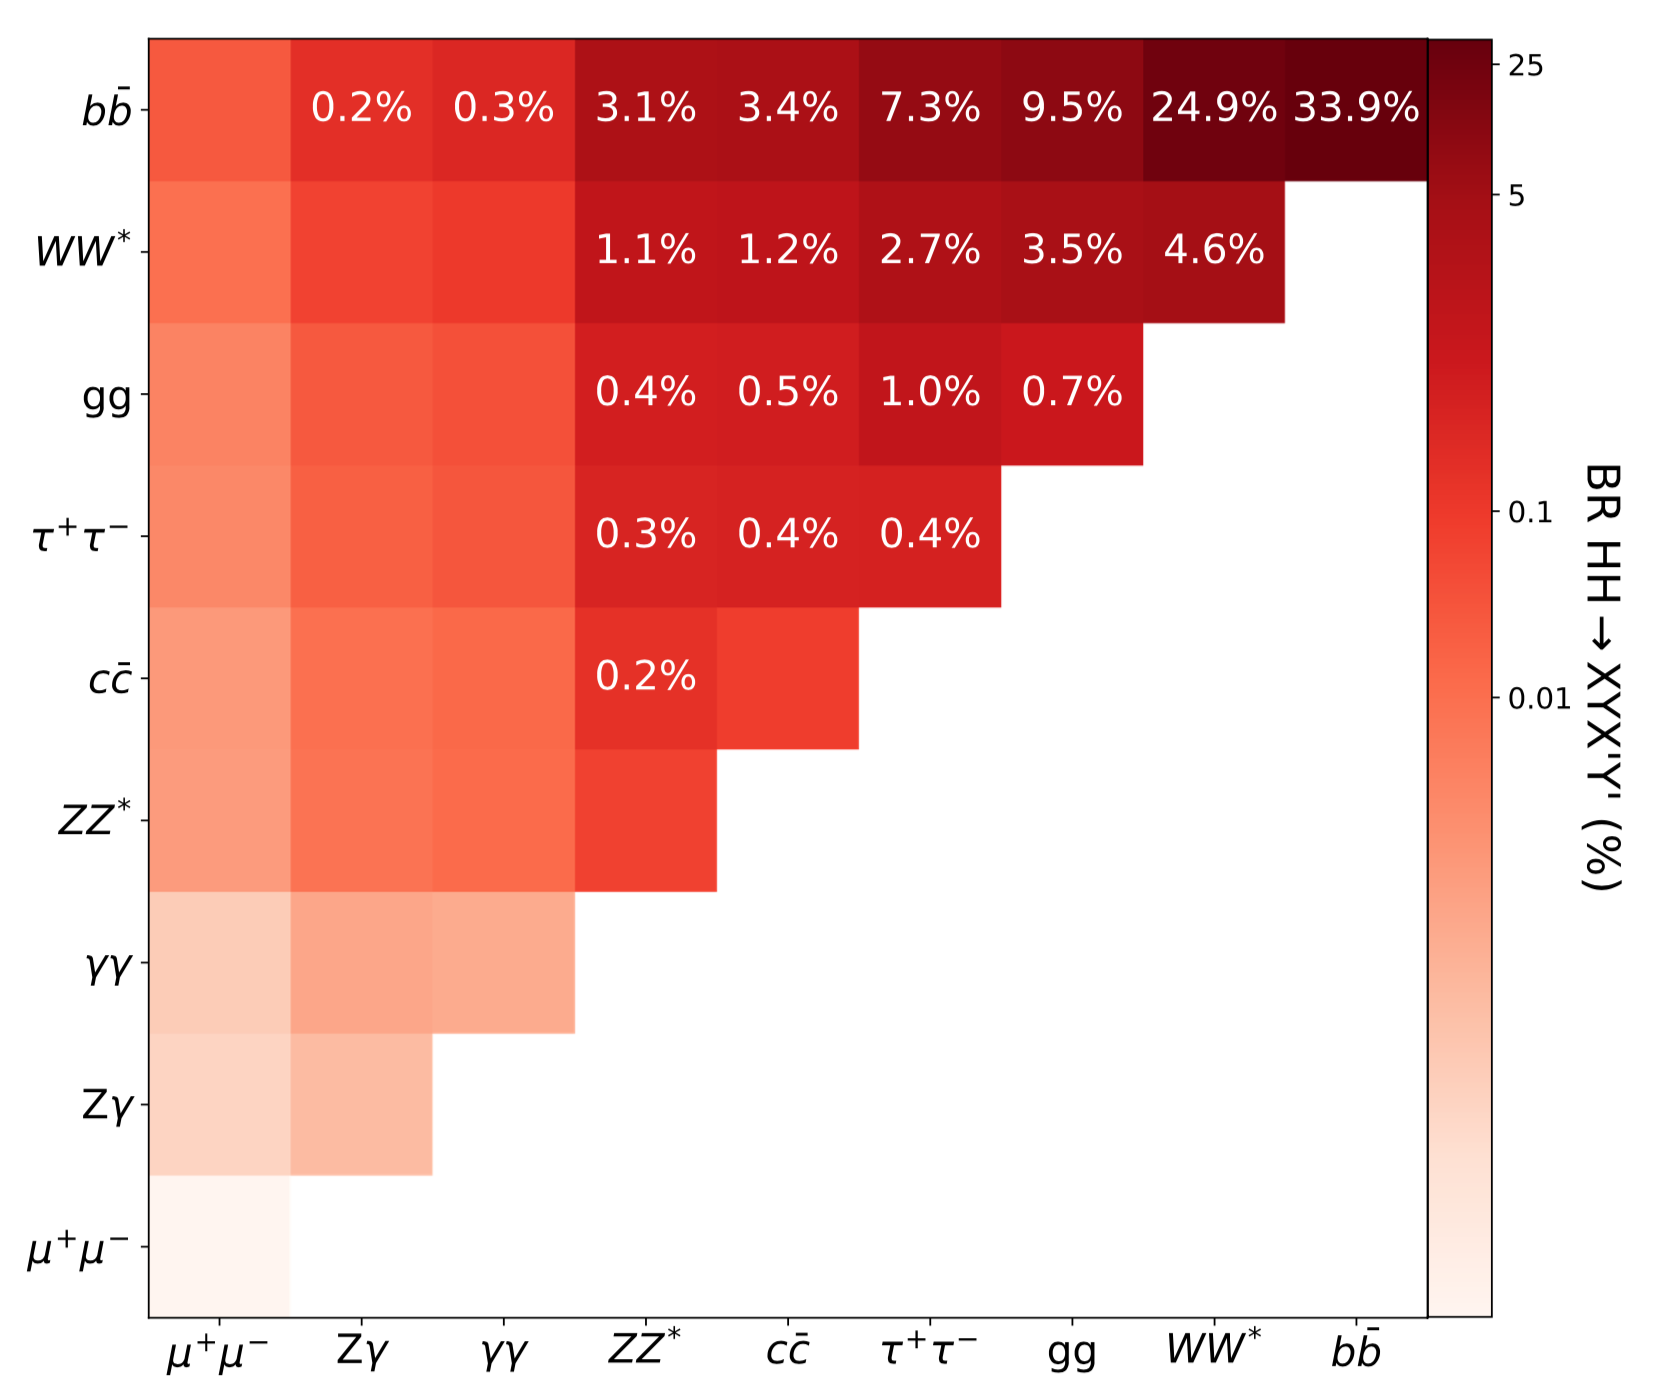
\includegraphics[width=.75\textwidth]{chapters/chapter1_theory/images/hh-brs.png}
    \caption[\gls{SM} Higgs boson branching ratios for $HH$ pairs to various final state combinations]{\gls{SM} Higgs boson branching ratios for $HH$ pairs to various final state combinations \cite{hh-whitepaper}.}
    \label{fig:hh-brs}
\end{figure}